\documentclass[../main.tex]{subfiles}
\begin{document}

\section{Topological Artist Model}
\label{sec:tam}
\begin{figure}[H]
    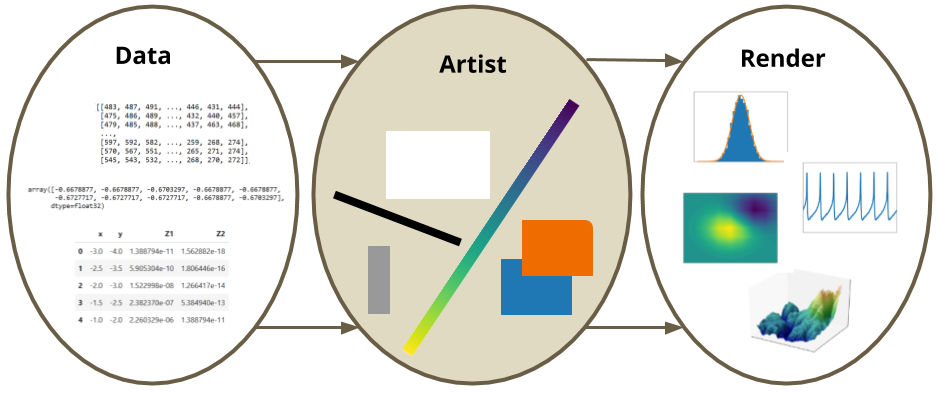
\includegraphics[width=\textwidth]{figures/math/dar.png}
    \caption{Visualizaiton is the process of mapping data into visual characteristics that are then assembled into a graphic}
    \label{fig:artist_stages}
\end{figure}

\note{can change this all to 3rd person passive later}\\
Visualization is generally thought of as structure preserving maps from data into graphics, and in this section we formally define that structure and how it is preserved via equivariant maps. We can then specify that a faithful visual mapping is structure preserving, and apply these constraints to visualizations we may want to develop or implement. We model the data, visual characteristic, and graphic stages of visualization, shown in figure~\ref{fig:artist_stages}, as topological structures that encapsulate types of variables and continuity; by doing so we can develop implementations that keep track of both in ways that let us distribute computation while still allowing assembly and dynamic update of the graphic. 

We introduce a mathematical description of the visualization pipeline where artist $\mathscr{A}$ functions transform data space $\mathscr{E}$ to an intermediate representation in a prerendered graphic space $\mathscr{H}$.

\begin{equation}
    \label{eq:artist}
    \mathscr{A}: \mathscr{E} \rightarrow \mathscr{H}
\end{equation}

We first describe how we model data(\ref{sec:data}), graphics(\ref{sec:graphic}), and intermediate visual characteristics (\ref{sec:artist}) as fiber bundles. We then discuss the equivariant maps between data and visual characteristics (\ref{sec:artist_nu}) and visual characteristics and graphics (\ref{sec:artist_q}) that make up the artist.

\subsection{Data Space}
\label{sec:data}
We build on Butler's proposal of using fiber bundles as a common data representation format for visualization data\cite{butlerVectorBundleClassesForm1992, butlerVisualizationModelBased1989} because fiber bundles are mathematical structures that are flexible enough express all the types of data described in section~\ref{sec:intro_data_structure}.

We model data as the fiber bundle $(E,\,B,\,\pi ,\,F)$, where $E$, $F$, and $K$ are topological spaces that encode 
\begin{itemize}
\item the properties of the variables in the fiber $F$ (\ref{sec:data_fiber})
\item the continuity of the records in the base space $K$ (\ref{sec:data_base})
\item collections of records $\tau$ (\ref{sec:data_section}). 
\end{itemize}

and $E$ is the total space of data that $F$ lives in. The bundle is the projection map $\pi$
\begin{equation}
    \label{eq:fiber_bundle}
    \begin{tikzcd}
        F \arrow[r, hook] & E \arrow[r, "\pi"] & K
    \end{tikzcd}
\end{equation}

that binds the variable space $F$ to the base space $K$. The fiber bundles mentioned in this work are assumed to be trivial\cite{spanier1989algebraic,LocallyTrivialFibre}, unless otherwise specified, because the trivial bundle is $E=K\times F$ such that extra structure in the total space $E$ falls out and discussion can be focused on the fiber and base space. 

\subsubsection{Variables: Fiber Space $F$}
\label{sec:data_fiber}
\note{yes, I know i may need to change this U to like $\mathcal{U}$, spivak uses U}
The fiber is a topological space that is the set of possible values of the data; the values themselves can be any dimension and type and have any continuity. We use Spivak's description of simplicial database schemas \cite{spivakSIMPLICIALDATABASES} as the basis of our fiber space because he binds the components of the fiber to variable names and types. Spivak constructs a set $U$ that is the disjoint union of all possible objects of types $\{T_0, \ldots, T_n\} \in DT$ where $DT$ are the data types of the variables in the dataset. He then defines the single variable set $U_\sigma$ 
\begin{equation}
    \label{eq:data_types}
\begin{tikzcd}
    U_{\sigma} \arrow[r] \arrow[d, "\pi_{\sigma}"'] & U \arrow[d, "\pi"] \\
    C \arrow[r, "\sigma"']                          & \textbf{DT}       
\end{tikzcd}
\end{equation}
which is $U$ restricted to objects of type $T$ bound to variable name $c$. Given $U_{\sigma}$, the fiber for a one variable dataset is
\begin{equation}
    F = U_{\sigma(c)} = U_{T} 
\end{equation}
where $\sigma$ is the schema binding variable name $c$ to its datatype $T$. A dataset with multiple variables has a fiber that is the cartesian cross product of $U_{\sigma}$ applied to all the columns:
\begin{equation}
F = U_{T_1}\times \ldots U_{T_i} \ldots\times U_{T_n}
\end{equation}

which is equivalent to 

\begin{equation}
    F= F_{0} \times \ldots \times F_{i}\times\ldots\times F_{n}
\end{equation}

which allows us to decouple $F$ into its component fibers $F_i$. For every variable
\begin{equation}
V_i = (c_i,\, T_i,\, U_{T_i})
\end{equation} 
we keep track of its name $c$, type $T$, and values $U_{T}$. 

\begin{figure}[H]
    \begin{subfigure}{.5\textwidth}
        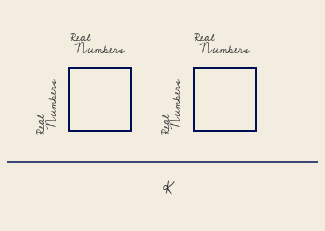
\includegraphics[width=\textwidth]{figures/math/temp_2f.png}
        \caption{}
        \label{fig:fiber_example_plane}
    \end{subfigure}
    \begin{subfigure}{.5\textwidth}
        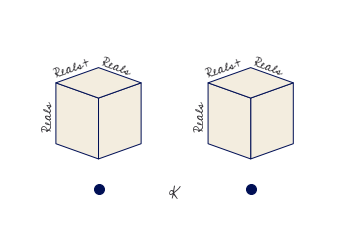
\includegraphics[width=\textwidth]{figures/math/temp_3f.png}
        \caption{}
        \label{fig:fiber_example_cube}
    \end{subfigure}
    \caption{These two datasets have the same base space $K$, but figure~\ref{fig:fiber_example_plane} has fiber  $F=\mathbb{R}\times\mathbb{R}^+$ which is (time, temperature) while figure~\ref{fig:fiber_example_cube} has fiber $\mathbb{R}^{+}\times\mathbb{R}^2$ which is (time, wind=(speed, direction))}
    \label{fig:data_fiber_example}
\end{figure}

For example, the data in figure~\ref{fig:fiber_example_plane} is a pair of times and \textdegree C temperature measurements taken at those times. Time is a positive number of type \texttt{detetime} which can be resolved to positive floats $U_{\texttt{datetime}}= \mathbb{R}^+$. Temperature values are real numbers $U_{\texttt{float}} = \mathbb{R}$. The fiber is 
\begin{equation}
    F =  \mathbb{R}^{+} \times \mathbb{R} 
\end{equation} 
where $V_0 = (time,\, \texttt{datetime},\, \mathbb{R}^+)$ and $V_1 = (temperature,\, \texttt{float},\, \mathbb{R})$. In figure~\ref{fig:fiber_example_cube}, temperature is replaced with wind. This wind variable is of type \texttt{wind} and has two components speed and direction $\{(s,d) \in \mathbb{R}^{2} \mid  0\leq s,\, 0 \leq d \leq 360\}$ . Therefore, the fiber is 
\begin{equation}
    F = \mathbb{R}^{+} \times \mathbb{R}^2
\end{equation} 
such that $V_1 = (wind,\, \texttt{wind},\, \mathbb{R}^{2})$  

\subsubsection{Measurement Scales: Monoid Actions}
\label{sec:data_monoid}
After specifying the variables $V$ in the dataset, we next describe ways in which we can transform the variables by identifying the monoid actions $M_i$ on the $F_i$. We use monoids as the abstraction because they encode composibilty, which maps well to the data transformation process in a software library \cite{yorgeyMonoidsThemeVariations}. 

A monoid \cite{Monoid2021} $M_i$ is a set with an associative binary operator $\ast:M_i \times M_i\rightarrow M_i$. A monoid has an identity element $e\in M_i$ such that $e\ast a= a \ast e = a$ for all $a \in M_i$. A left monoid action \cite{SemigroupAction2021,ActionNLab} of $M_i$ is a set $F_i$ with an action $\bullet: M\times F_i \rightarrow F_i$ with the properties:
\begin{align*}
    \textbf{associativity}\;& \text{for all } f,g \in M_i \text{ and } x\in F_i,\, f\bullet(g\bullet x) = (f\ast g) \bullet x\\
    \textbf{identity}\;& \text{for all } x\in F_i, e\in M_i,\,  e\bullet x = x 
\end{align*}
As with the fiber $F$, the total monoid space $M$ is the cartesian product
\begin{equation}
M = M_{0} \times \ldots \times M_{i}\times \ldots \times\ldots M_{n}
\end{equation}
of the monoid $M_{i}$ on each $F_{i}\in F$. We expand our definition of variables 
\begin{equation}
        V_i = (c_i,\, T_i,\, F_i\, M_i)
\end{equation}
to include the monoid actions that act on $F_i$. 

Steven's described the measurement scales\cite{stevensTheoryScalesMeasurement1946,leaFormalizationMeasurementScale} in terms of the monoid actions on the measurements: nominal data is permutable, ordinal data is monotonic, interval data is translatable, and ratio data is scalable \cite{weissteinSimilarityTransformation}. For example, given  $V_0 = (temperature,\, \texttt{float},\, \mathbb{R})$ which is interval data:
\begin{itemize}
    \item monoid operator addition $\ast = +$
    \item monoid operations: $f: x\mapsto x + c_1 $, $g: x\mapsto x + c_2$
    \item monoid action operator composition $\bullet = \circ$
\end{itemize}
then the translation monoid actions on temperature satisfy the condition
\begin{equation}
    \begin{tikzcd}
        \mathbb{R} \arrow[rd, "(x+c_1)\circ(x+c_2)"] \arrow[d, "x+c_1"'] &            \\
        \mathbb{R} \arrow[r, "x+c_2"']                                   & \mathbb{R}
    \end{tikzcd}
\end{equation}
where $c_1, c_2$ are intervals $x_i-x_j$. 


\subsubsection{Continuity: Base Space $K$} 
\label{sec:data_base}
The advantage of fiber bundles is they provide a way to encode the continuity in a dataset as the basespace $K$ without making assumptions as to what that continuity is. In turn this representation of continuity can then be used to keep track of how the data fits together, for example if a visualization of a very large dataset calls for parallelization.  

\begin{figure}[H]
    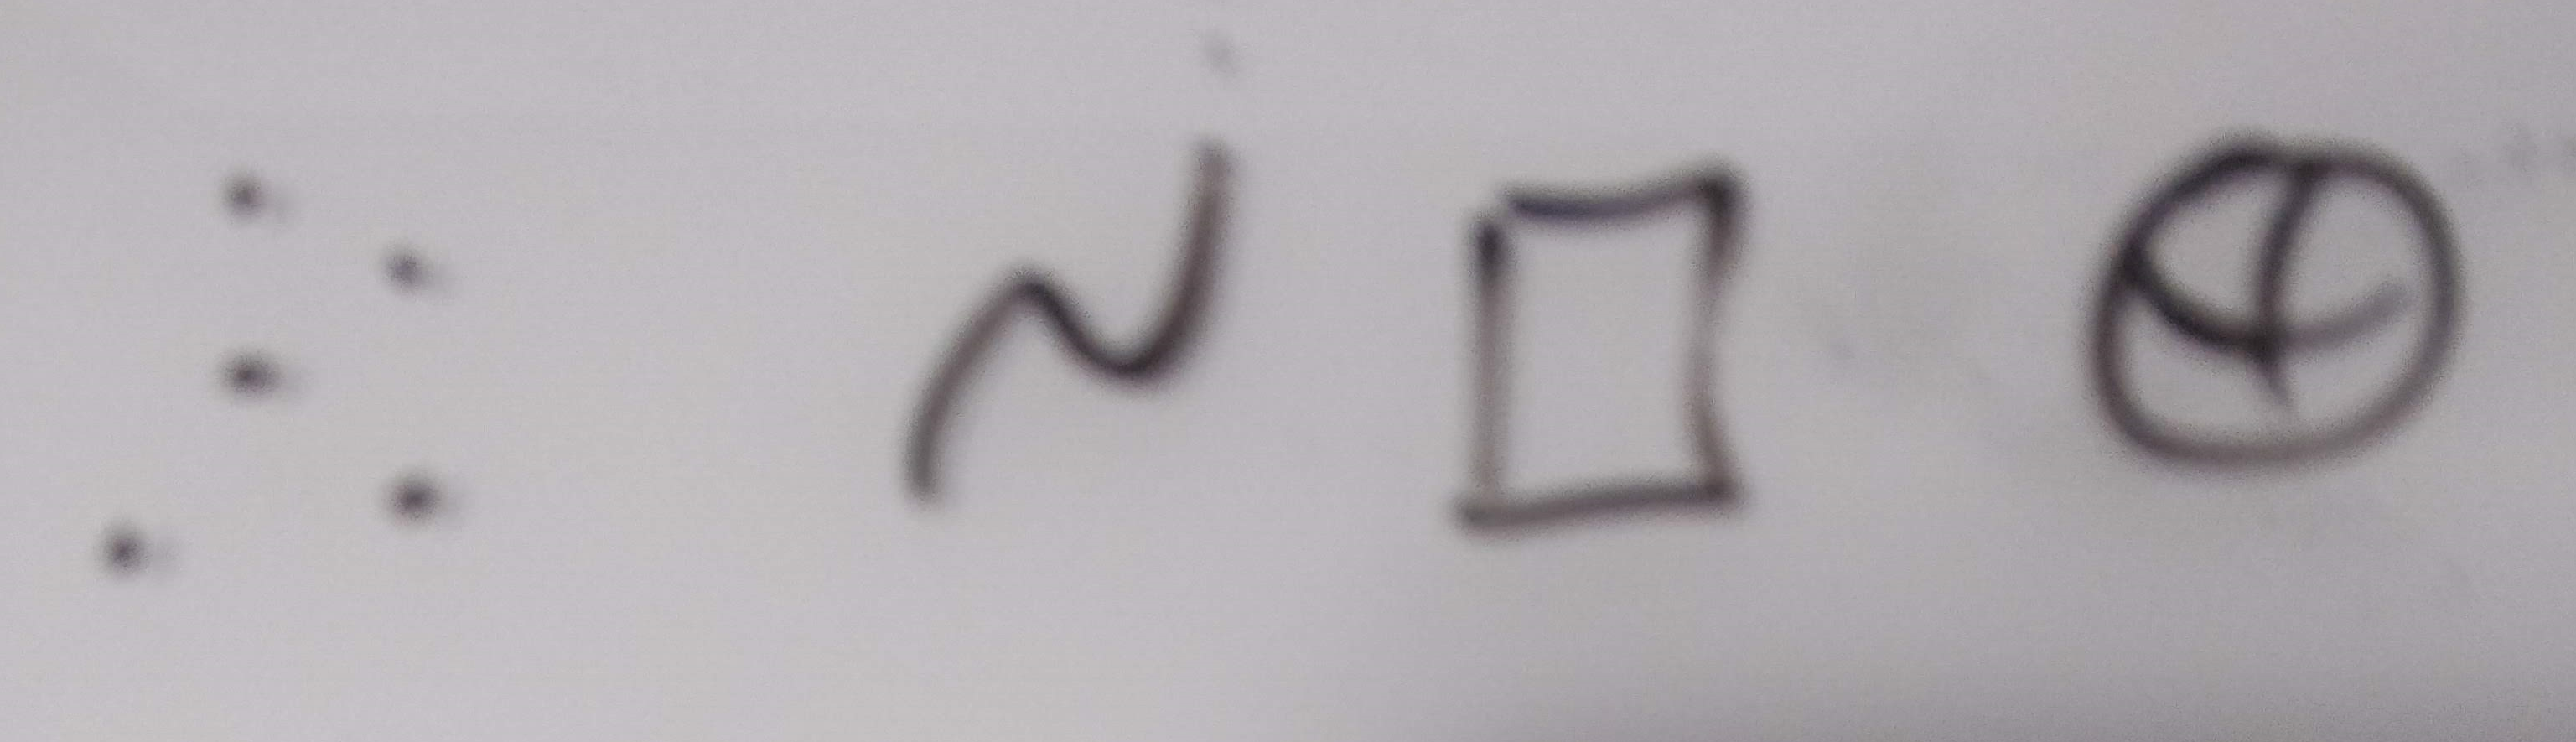
\includegraphics[width=.5\textwidth]{figures/math/k_different_types.png}
    \caption{The topological base space $K$ encodes the connectivity of the data space, for example if the data is independent points or a map or on a sphere}
    \label{fig:base_space_types}
\end{figure}
As illustrated in figure~\ref{fig:base_space_types}, $K$ is akin to an indexing space into $E$ that describes the structure of $E$.  $K$ can have any number of dimensions and be continuous or discrete. 

\begin{figure}[H]
    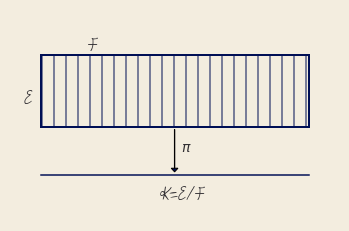
\includegraphics[width=.5\linewidth]{figures/math/k_qspace.png}
    \caption{The base space $E$ is divided into fiber segments $F$. The base space $K$ acts as an index into the records in the fibers.
    \note{this figure might be good all the way up top to lay out the components of fb}}
    \label{fig:base_space_div}
\end{figure}

Formally $K$ is the quotient space \cite{QuotientSpaceTopology2020} of $E$, meaning it is the finest space\cite{aurouxMath131Introduction} such that every $k \in K$ has a corresponding fiber $F_k$ in $E$\cite{QuotientSpaceTopology2020}. In figure~\ref{fig:base_space_div}, $E$ is a rectangle divided by vertical fibers $F$, so the minimal $K$ for which there is always a mapping $\pi: F\rightarrow K$ is the line. 

As with fibers and monoids, we can decompose the total space into components $\pi:E_i\rightarrow K$ where
\begin{equation}
    \pi:E_1\oplus\ldots\oplus E_i \oplus\ldots \oplus E_n \rightarrow K
\end{equation}

which is a decomposition of $F$. The $K$ remains the same because the connectivity of records 
does not change just because there are fewer elements in each record.

\begin{figure}[ht!]
    \begin{subfigure}{.5\textwidth}
        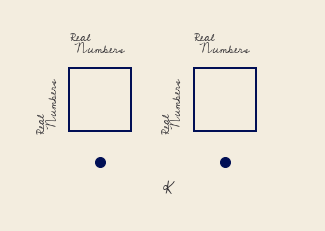
\includegraphics[width=\textwidth]{figures/math/temp_1k.png}
        %% add box around neighboring P and Map
        \caption{}
        \label{fig:base_example_discrete}
    \end{subfigure}
    \begin{subfigure}{.5\textwidth}
        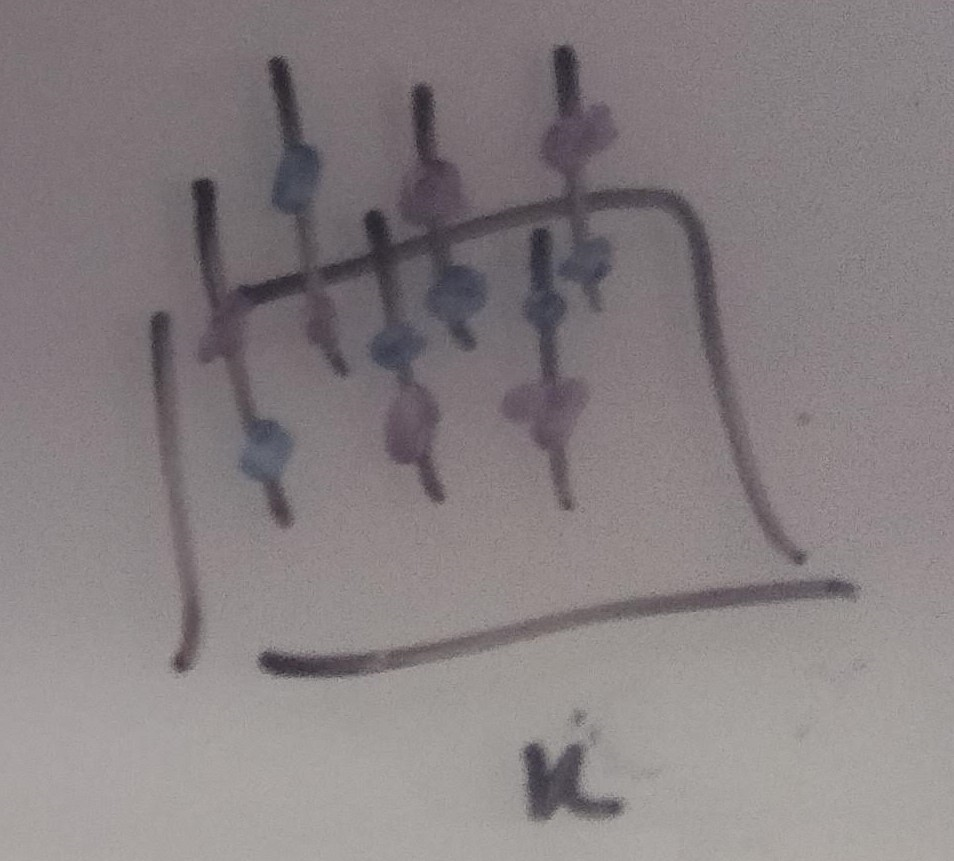
\includegraphics[width=\textwidth]{figures/math/temp_2k.png}
        \caption{}
        \label{fig:base_example_continuous}
    \end{subfigure}
    \caption{These two datasets have the same (time, temperature) fiber. In figure~\ref{fig:base_example_line} the total space $E$ is discrete over points $k \in K$, meaning the records in the fiber are also discrete. In figure~\ref{fig:base_example_plane} $E$ lies over the continuous interval $K$, meaning the records in the fiber are sampled from a continuous space. 
    \note{revamp figure: F=Plane, k1 = dots, k2=line}}
    \label{fig:base_example}
\end{figure}

The datasets in figure~\ref{fig:base_example} have the same fiber of (temperature, time) which is $F=\mathbb{R}\times \mathbb{R}^+$. In figure~\ref{fig:base_example_discrete} the fibers lie over discrete $K$ such that the records in the datasets in the fiber bundles are discrete. The same fiber in figure~\ref{fig:base_example_continuous} lies over a continuous interval $K$ such that the records are samples from a continuous function defined on $K$.

\subsubsection{Data: Sections $\tau$}
\label{sec:data_section}
While the fiber and base space describe the general structure of all data that lives in the fiber bundle, the sections $\tau: K\rightarrow E$ define the datasets that live in the fiber. We generalize Spivak's section as table $\tau$\cite{spivakSIMPLICIALDATABASES} to any sort of structured dataset such that 
\begin{equation}
    \begin{tikzcd}
        F \arrow[r, hook] & E \arrow[d, "\pi"']              \\
                          & K \arrow[u, "\tau"', bend right]
    \end{tikzcd}
\end{equation}
such that there is $\pi(\tau(k)) = k$ map back to $K$. There can be many sections $\tau$, and the space of global sections is $\Gamma(E)$. For a trivial fiber bundle
\begin{equation}
    \label{eq:section_return}
    \tau(k) = (k, (g_{F_{0}}(k), \ldots, g_{F_{n}}(k))
\end{equation}
where $g: K \rightarrow F$ is the index function into the fiber. Because we can decompose the bundle and the fiber, we can formulate $\tau$ as 
\begin{align}
\tau = (\tau_0,\ldots, \tau_i, \dots, \tau_n) 
\end{align}
where each section $\tau_i$ is a variable or set of variables. 

\begin{figure}[H]
    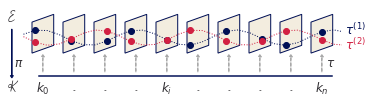
\includegraphics[width=.5\linewidth]{figures/math/fiberbundle.png}
    \caption{ Fiber (time, temperature) with an interval $K$ basespace. The sections $\tau_1$ and $\tau_2$ are constrained such that the time variable must be monotonic, which means each section is a timeseries of temperature values. They are included in the global set of sections  $\tau_1, \tau_2 \in \Gamma(E)$}
    \label{fig:data_sections}
\end{figure}

In the example in figure~\ref{fig:data_sections}, the fiber is $\mathbb{R}^+\times \mathbb{R}$ as described in figure~\ref{fig:data_fiber_example} and the base space is the interval $K$. The section $\tau_1$ resolves to a series of monotonically increasing in time records of temperature. Section $\tau_2$ returns a different timeseries of temperature values. Both sections are included in the global set of sections $\tau_1, \tau_2 \in \Gamma(E)$.

\subsubsection{Sheaf and Stalk}
\label{sec:data_sheaf_stalk}
Often a graphic may need to be updated with live data or support zooming in on a segement of the dataset; to support working with a subset of data, we can use the sheaf $\mathcal{O}(E)$. All fiber bundles are locally trivial, which means that $E$ restricted over a small enough neighborhood $U \subset K$ is a locally trivial bundle over $U$\cite{LocallyTrivialFibre}. The sheaf $O(E)$ is the localized section of fibers $\iota^*\tau: U \rightarrow \iota^*E$

\begin{equation}
    \label{eq:sheaf}
    \begin{tikzcd}
        \iota^*E \arrow[d, "\pi"']           & E \arrow[d, "\pi"'] \arrow[l, "\iota^*"']         \\
        U \arrow[u, "\iota^*\tau"', bend right] & K \arrow[u, "\tau"', bend right] \arrow[l, "\iota"']
        \end{tikzcd}
\end{equation}
pulled back over the neighborhood $U$ via the inclusion map $\iota: U \rightarrow K$. The localized section is the germ $\xi^*\tau$. The neighborhood of points $k_i$ surrounding the point $k$ the sheaf lies over is the stalk $\mathcal{F}_b$ \cite{StalkSheaf2019,spanier1989algebraic}. While $E$ is only the records in a fiber $F_k$ over a specific $k$, because the stalk includes the neighborhood $U$ it also includes nearby records. While this can be useful for visual transforms, often the extra needed information can be found in the jet bundle $\mathcal{J}$ \cite{JetBundle2020,musilovaCalculusVariationsJet2016}. For example, line thickness requires the derivative of the given position to be rendered, which can be found in $E^\prime=E+\mathcal{J}(E)$


\subsection{Graphic: $H$}
\label{sec:graphic}  
We can separate the structure of the graphic from the properties of the output format by modeling the space of graphics as a fiber bundle  $(H, S, \pi, D)$. As with data, the fiber bundle is for a class of graphics with shared base space $S$ (~\ref{sec:graphic_fiber}) and fiber $D$ (~\ref{sec:graphic_base}) and the sections $\rho$ (~\ref{sec:graphic_section}) encode the fully specified graphics. 

\subsubsection{Idealized Display $D$}
\label{sec:graphic_fiber}
% infinite resolution version of D
The fiber $D$ is specified in terms of the target display space, for example a 2D screen or 3D printer. In this work, we assume a 2D opaque image $D=\mathbb{R}^5$ with elements in $D$ of the form
\begin{equation}
    d = (x, y, r, g, b)
\end{equation}
such that a rendered graphic only consists of 2D position and color. To support overplotting and transparency, the fiber could be $D=R^{7}$ such that $d=(x, y, z, r, g, b, a)$. The location coordinates $x$ and $y$ are defined in terms of the display, while the $(r,g,b)$ values are filled in via a lookup on $S$. 

\subsubsection{Continuity of the Graphic $S$} 
\label{sec:graphic_base}
An assumption of graphical representations is that they match the continuity of the data\cite{tufteVisualDisplayQuantitative2001,friendlyBriefHistoryData2008}, but the underlying topology $S$ of a graphic may need more dimensions than the data topology $K$ so that the glyph can be defined in $D$. Therefore we define the base space mapping from graphic $S$ to data $K$ 
\begin{equation}
    \begin{tikzcd}
        E \arrow[d, "\pi"'] & H \arrow[d, "\pi"'] \\
        K                   & S \arrow[l, "\xi"']
        \end{tikzcd}
\end{equation}

 as the deformation retraction \cite{RetractionTopology2020} $\xi: S \rightarrow K$ that goes from a region $s \in S_{k}$ to its associated point $k$, such that when $\xi(s) = k$, $\xi^*\tau(s) = \tau(k)$. While dimensions can be added to $S$, it retains the same continuity as $K$.
 
\begin{figure}
    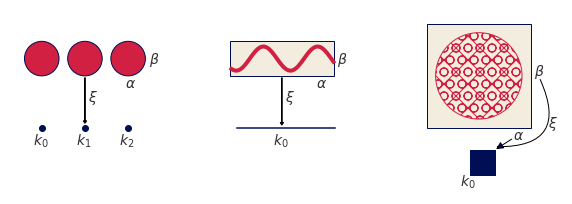
\includegraphics[width=1\textwidth]{figures/math/retraction_maps.png}
    \caption{The scatter and line graphic base spaces $S$ are larger than $K$ so that they can encode physical aspects of the glyph, such as shape (a circle) or thickness. The heatmap base $S$ is the same as $K$ because a heatmap is directly mapping the values in the data to the graphic.
    \note{add $\alpha, \beta$ coordinates}}
    \label{fig:graphic_retraction_map}
\end{figure}

In figure~\ref{fig:graphic_retraction_map} each disk $S_k$ indexes how elements in $D$ are held together to generate a single glyph that is the visual representation of a single point in $F_k$. For the line, the region $\beta$ over a point $\alpha_i$ specifies the thickness of the line in $D$ for the corresponding section on the interval $K$. The heatmap has the same continuity in data space and graphic space such that no extra dimensions are needed. 

 
\subsubsection{Renderable Glyph $\rho$}
\label{sec:graphic_section}
%pick a pixel which is the bounding box
A section $\rho: S\rightarrow H$ defines a piece of the graphical representation of the data. The physical display coordinates in $D$ are not equivalent to the mathematical coordinates in $S$ such that many points $s \in S$ might map to a single $d\in D$ and many $d$ might go into a visible section of a displayed graphic. Therefore, we define the bounding box $b=\left[y_{top}, y_{bottom}, x_{right}, x_{left}\right]$ in the display space $D$ that is a piece of the rendered graphic.  

We inverse map this bounding box $S_b =\rho^{-1}(b)$ into a region $S_b \subset S$  
\begin{align}
    R_b &= \iint\limits_{S_b} \rho_r(s)ds^{2}\\
    G_b &= \iint\limits_{S_b} \rho_g(s)ds^{2}\\
    B_b &= \iint\limits_{S_b} \rho_b(s)ds^{2}
\end{align}
to then compute the remaining $(R, G, B)$ components of the bounded display region $D_b$.

\begin{figure}
    \includegraphics[width=\textwidth]{figures/math/graphic_render.png}
    \caption{To render a graphic, a region $b$ is selected in the display space. This region is in coordinates $D$ so the inverse mapping $\rho^{-1}(b)$ maps to an equivalent region $S_b \subset S$. We then take the sections $\rho(S_b)$ which are the elements $\{d_0, \ldots, d_n\}$ that make the piece of the graphic in $b$.}
    \label{fig:graphic_rho_lookup}
\end{figure}
As shown in figure~\ref{fig:graphic_rho_lookup}, the output space queries into the graphic bundle to render the image. We select a region $b$ in the output space, inverse map the region into $S_b \subset S$, then take the section $\rho$ over the region $S_b$. The section yields the set of elements $\{d_0, \ldots, d_n\}$ that specify the $(r, g, b)$ values corresponding to the coordinates in $b$. 

\subsection{Artist}
\label{sec:artist}
\begin{figure}[H]
    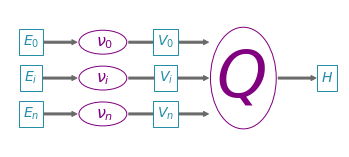
\includegraphics[width=\textwidth]{figures/math/path_of_q}

    \caption{The $\nu$ functions convert data $E$ to visual $V$. $Q$ assembles the different types of visual parameters $V_{i}$ into a graphic in $H$. $Q\circ\mu(\xi^{-1}J)$ forms a visual mark by applying $Q$ to a region mapped to connected components $J \subset K$. \note{maybe change to $\tau, \mu, \rho$ }} 
    \label{fig:artist_q}
\end{figure}

The artist is the function that converts data into graphics; its name is taken from the analogous part of the existing Matplotlib architecture that builds visual elements to pass off to the renderer. The artist is a mapping from $E$ padded with data from $\mathcal{J}(E)$ to a graphic that is a section $\rho$ in  $\Gamma(H)$
\begin{equation}
    \label{eq:artist_diagram}
    \begin{tikzcd}
        E' \arrow[r, "\nu"] \arrow[rd, "\pi"'] & V \arrow[d, "\pi"] & \xi^*V \arrow[r, "Q"] \arrow[d, "\xi^*\pi"'] \arrow[l, "\xi^*"'] & \Gamma(H) \arrow[ld, "\pi"] \\
                                              & K                  & S \arrow[l, "\xi"']                                              &                    
        \end{tikzcd}
\end{equation}
with an intermediate fiber bundle $V$ to hold visual representations and stages
\begin{enumerate}
    \item $\xi$ binding the continuity in the graphic to the continuity in the data (~\ref{sec:graphic_base})
    \item $\nu$ conversion of data into visual characteristics (~\ref{sec:artist_nu})
    \item $Q$ assembly of visual variables into a glyph (~\ref{sec:artist_q})
\end{enumerate}
 
of the visual transformation illustrated in figure~\ref{fig:artist_stages}. The functions $\xi$, $\nu$ and $Q$ are constructed such that the input can be a single section on $K$ or $S$, which allows the artist to be trivially parallelized or formulated as a delayed computer graph or otherwise not need to immediately work on all the data. 

\subsubsection {Visual Fiber Bundle $V$}
The visual fiber bundle ($V$, $K$, $\pi$, $P$) has section $\mu: V \rightarrow K$ that resolves to a visual variable \cite{bertinIIPropertiesGraphic2011,munznerMarksChannels} in fiber $P$. The fiber space $P$ is defined in terms of the parameters of the visualization specification and the values those parameters resolve to - for example ggplot \cite{wickhamGgplot2ElegantGraphics2016a} or D3\cite{bostockDataDrivenDocuments2011}.
\begin{table}[H]
    \renewcommand{\arraystretch}{2}
    \begin{tabulary}{\textwidth}{|l|L|l|}\hline
     $\bm{\nu_{i}}$                      & $\bm{\mu_{i}}$                                                            & $\bm{codomain(\nu_{i})}$  \\ \hline                                              
    position                    & x, y, z, theta, r                                                          & $\mathbb{R}$   \\ \hline
    size                        & linewidth, markersize                                            & $\mathbb{R}^{+}$   \\ \hline
    shape                       & markerstyle                                                      & $\{f_{0}, \ldots, f_{n}\}$ \\ \hline
    color                       & color, facecolor, markerfacecolor, edgecolor  & $\mathbb{R}^{4}$ \\ \hline
    \multirow{2}{*}{texture}    & hatch                                                            & $\mathbb{N}^{10}$\\\cline{2-3}
                                & linestyle                                                        & $\{f_{0}, \ldots, f_{n}\} \times (\mathbb{R}, \mathbb{R^+}^{n, n\%2=0})$ \\ \hline              
    \end{tabulary}
    \caption{Some possible components of the fiber $P$ for a visualization implemented in Matplotlib}
    \label{tab:mpl_visual_variable_fiber}
\end{table}

Table~\ref{tab:mpl_visual_variable_fiber} is a sample of the fiber space for Matplotlib \cite{hunterMatplotlib2DGraphics2007}. A section $\mu$ of $V$ is a tuple of visual values that specifies the visual characteristics of a part of the graphic. For example, given a fiber of $\{xpos, ypos, color\}$ one possible section could be  $\{.5, .5, (255, 20,147)\}$. The $codomain(\nu_i)$ determines the monoid actions on $\mu_i)$. These fiber components are implicit in the library, by making them explicit as components of the fiber we can build consistent definitions and expectations of how these parameters behave. 

\subsubsection{Visual Channels}
\label{sec:artist_nu}
\begin{figure}[H]
    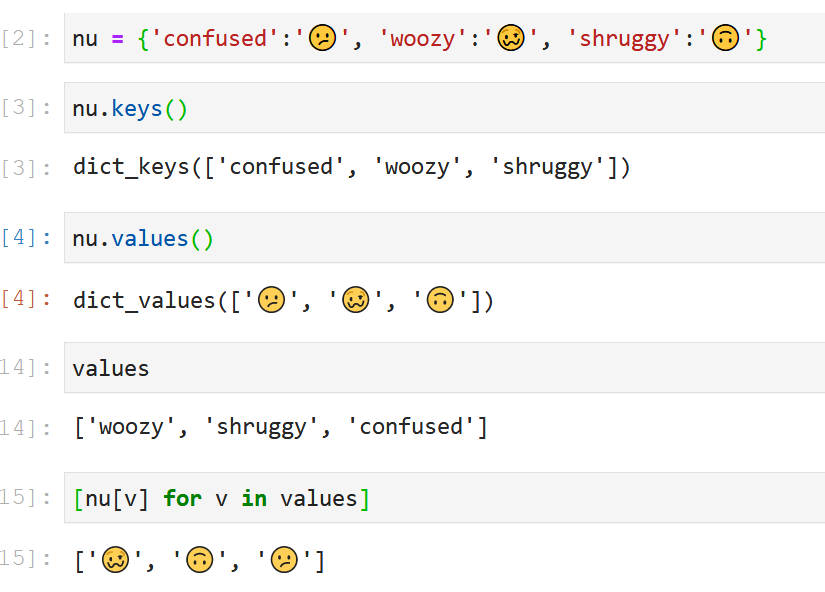
\includegraphics[width=\textwidth]{figures/math/equivariance_nu.png}
    \caption{An equivariant $\nu$ preserves monoid actions. Here $\nu$ maps the words to the emojis and is constructed such that a permutation of the words is reflected in a permutation of the symbols. \note{will switch to a figure table thing but this is the idea}}
    \label{fig:artist_nu}
\end{figure}
As introduced in section~\ref{sec:intro_visual_variables}, there are many ways to encode data visually. We define the visual transformers $\nu$ as the set of conversion functions 
\begin{equation}
    \label{eq:nu_expanded}
    \{\nu_{0}, \ldots, \nu_{n}\}: \{\tau_{0}, \ldots, \tau_{n}\} \mapsto \{\mu_{0}, \ldots, \mu_{n}\}
\end{equation}
such that $\nu_i: \tau_i \mapsto \mu_i$ is an equivariant map such that there is a monoid homomorphism from $F_{i}$ to $V_{i}$. A validly constructed $\nu$ is one where the  diagram 
\begin{equation}
    \label{eq:nu_categorical}
\begin{tikzcd}
    E_i \arrow[r] \arrow[r, "\nu_i"] \arrow[d, "m_e"'] & V_i \arrow[d, "m_v"] \\
    E_i \arrow[r, "\nu_i"]                           & V_i               
\end{tikzcd}
\end{equation}
commutes such that $\nu_i(m_e(E_i)) = m_v(\nu_i(E_i))$. This equivariance constraint yields guidance on what makes for an invalid transform. For example, the single value conversion $\nu_{i}(x) = .5$ does not commute under translation  $t(x) = x+2$  
\begin{align}
    \nu(t(e + 2)) & \overset{?}{=} \nu(e) + \nu(2)\\
    .5 &\neq .5 + .5
\end{align}

On the other hand figure~\ref{fig:artist_nu} illustrates a valid $\nu$ mapping from \textbf{Strings} to symbols. The group action on these sets is permutation, so shuffling the words must have an equivalent shuffle of the symbols they are mapped to. To preserve ordinal and partial order monoid actions, $\nu$ must be a monotonic function such that given $e_1, e_2 \in E_{i}$, $\text{ if } e_1 \leq e_2 \text{ then } \nu(e_1) \leq \nu(e_2)$. For interval scale data, $\nu$ is equivariant under translation monoid actions if $\nu(x + c) = \nu(x) + \nu(c)$. For ratio data, there must be equivalent scaling $ \nu(xc) = \nu(x)\nu(c)$.

\subsubsection{Assembling Marks}
\label{sec:artist_q}

As shown in figure~\ref{fig:artist_q}, $Q$ takes the individual fields in $V$ as input and outputs a single piece of a graphic on $H$. As with $\nu$, the constraint on $Q$ is that for every monoid actions on the input in $V$ there is a corresponding monoid action on the output in $H$
\begin{equation}
    Q: \Gamma(V) \rightarrow \Gamma(H)
\end{equation}
When $Q: \mu \mapsto \rho$ yields a $\rho$ that maps to the same values in $D$ over all $S_k$, then $M$ can be defined over $\Gamma(H)$ such that a constraint on $Q$ is that it must be equivariant. For example, when $\mu_{i}$ is the color of the glyph, it maps directly to (R,G,B) in D.

\begin{figure}[H]
    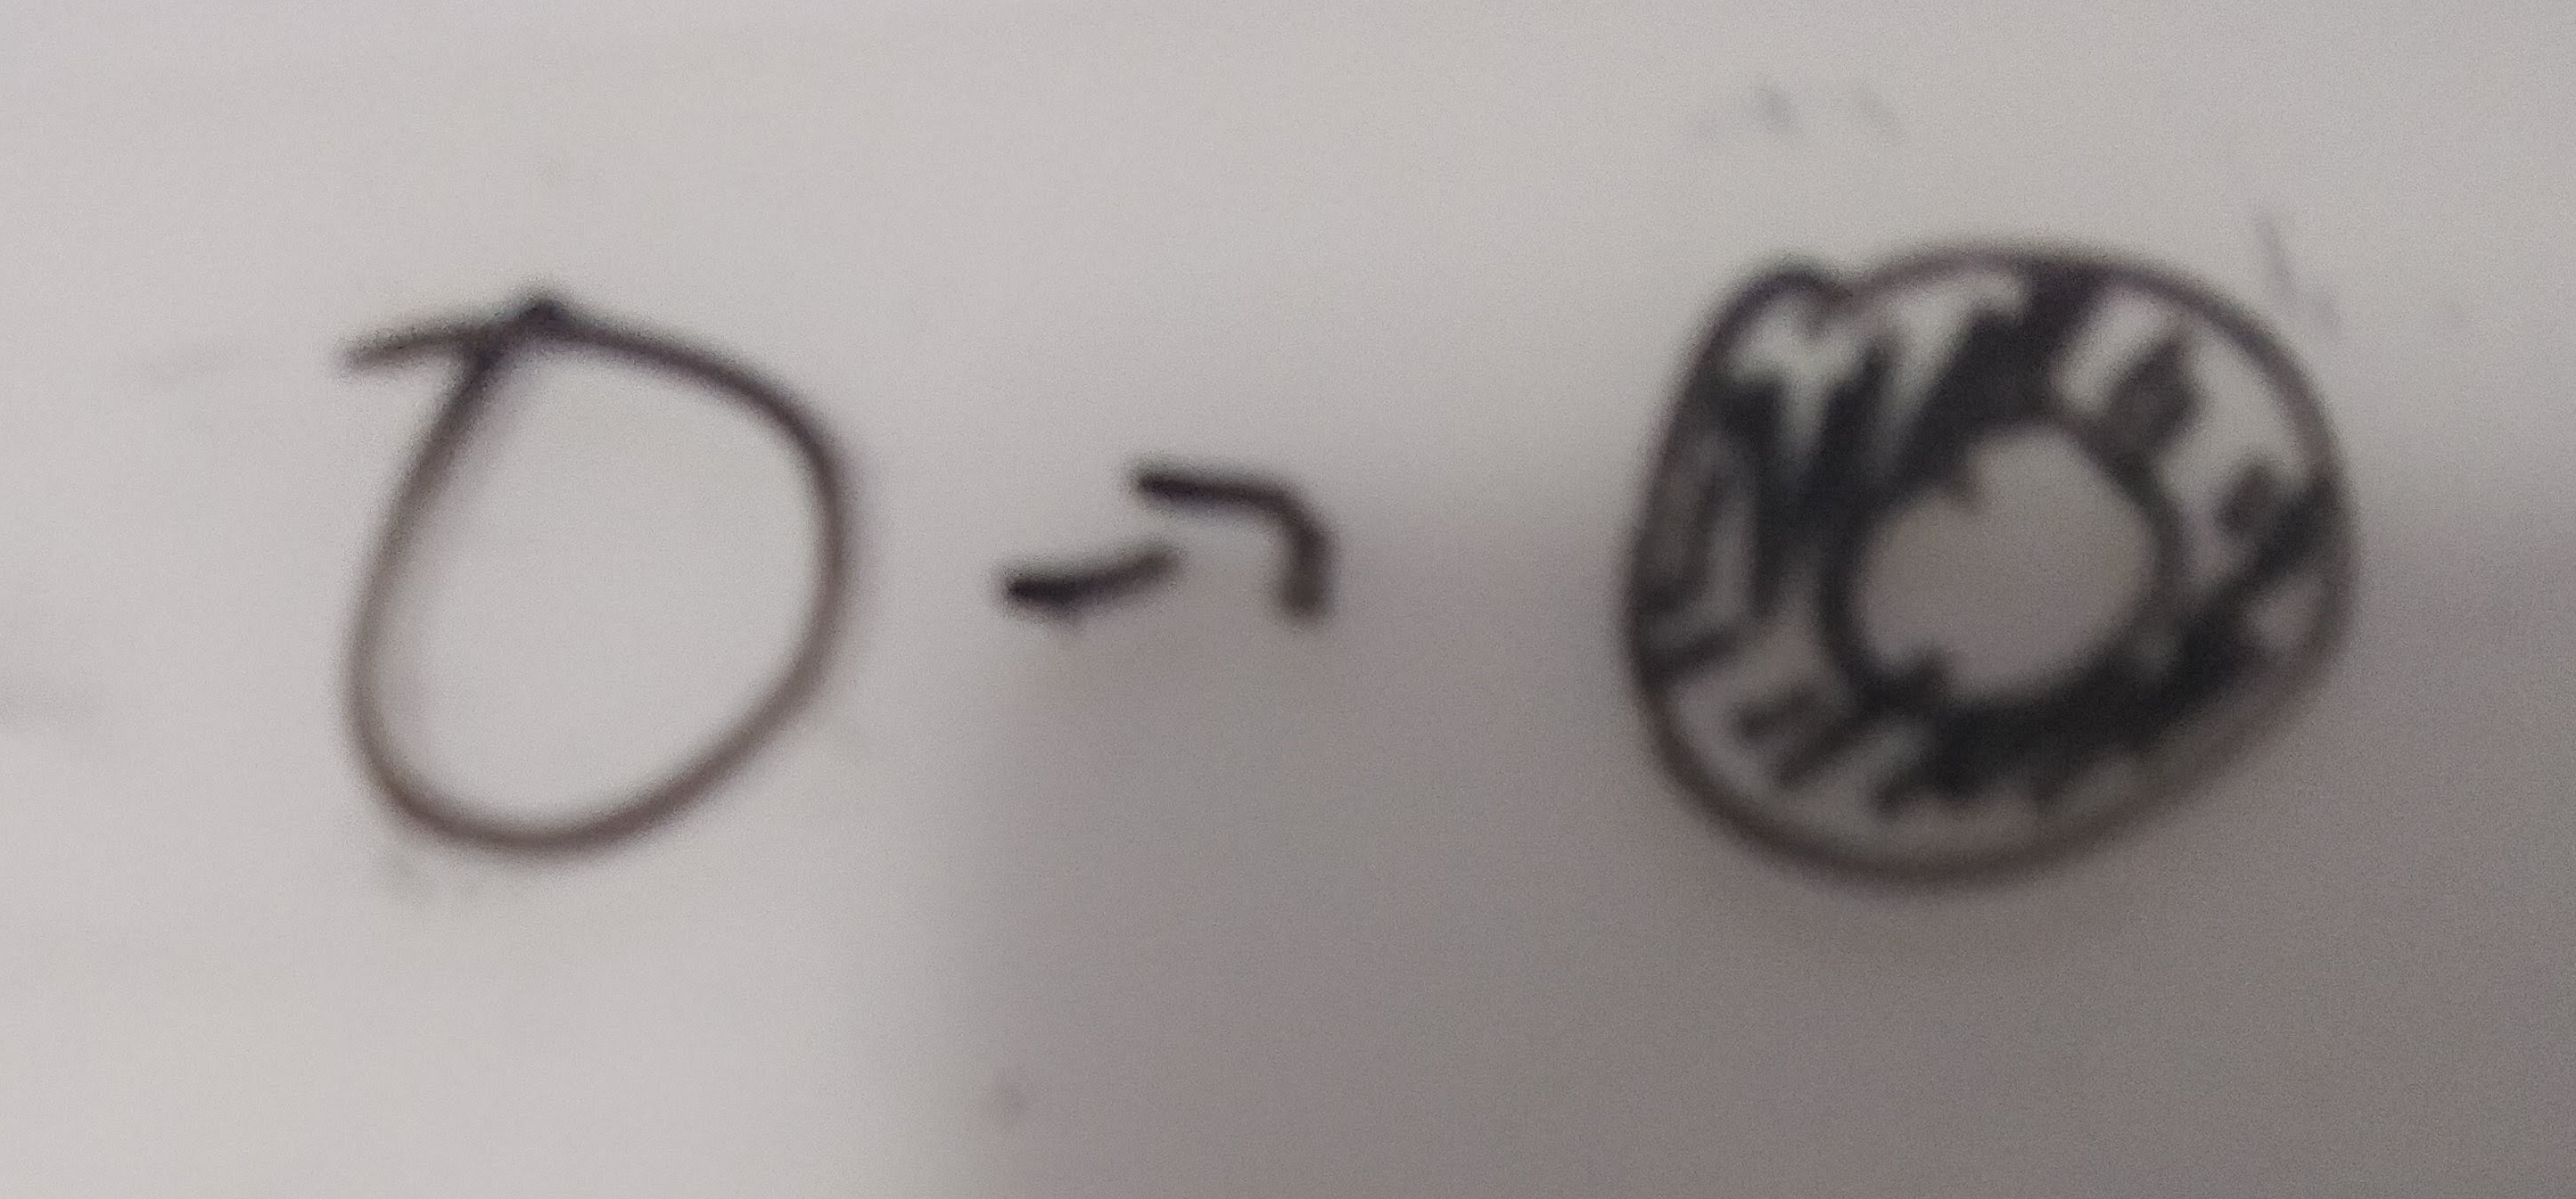
\includegraphics[width=\textwidth]{figures/math/diff_type_q.png}
    \label{fig:artist_mark_change}
\end{figure}

Many $\mu_{i}$ are graphical parameters that do not apply to the whole glyph, such as edge thickness in figure~\ref{fig:artist_mark_change}. 

%%% rework this sentence
In these situations, not all  $\rho$ in $\Gamma(H)$ will support these parameters; instead we define an action on the output graphic $Q(\Gamma(V)) \in \Gamma(H)$ since by definition every section $\mu$ will have a corresponding $\rho$.

We then define the constraint on $Q$ such that if $Q$ applied to two sections $\mu, \mu\prime$ generate the same graphic $\rho$, then the output of both sections acted on by the same monoid $m$ must also be the same.    

Lets call the visual encodings $\Gamma(V)=X$ and the graphic $Q(\Gamma(V))=Y$. If $\forall m \in M$ and $\forall \mu, \mu^\prime \in X$, 
\begin{equation}
Q(\mu) = Q(\mu^\prime)\implies Q(m\circ\mu) = Q(m\circ\mu^\prime)
\end{equation}
then a group action on $Y$ can be defined as $m\circ \rho = \rho^\prime$ where $\rho^\prime=Q(g\circ \mu)$ with $\mu \in Q^{-1}(\rho)$. 

Given  
\begin{itemize}
    \item $P = \{xpos, ypos, color, thickness\}$
    \item $\mu = {0,0,0, 1}$
    \item  $Q(\mu)=\rho$ generates a piece of the thin circle in figure~\ref{fig:artist_mark_change}
\end{itemize}

the constraint on $Q$ means that the translation $m=\{e, e, e, x+2\}$ applied to $\mu$ such that $\mu^\prime=\{0,0,0,3\}$ has an equivalent action on $\rho$ that causes $Q(\mu\prime)$ to be equivalent to the thicker circle in figure~\ref{fig:artist_mark_change}.


\paragraph{Example: Invalid Q}
\textcolor{blue}{Insert some degenerate Q that generates an inconsistent glyph}


Check a well defined map $M\times Y \rightarrow Y$.


constraint: inputs go to same o
utput means changes to inputs mean same changes to output

\paragraph{Graphical Marks}
To output a mark  \cite{bertinIIPropertiesGraphic2011,carpendaleVisualRepresentationSemiology}, $Q$ is called with all the regions $s$ that map back to a set of connected components $J \subset K$:
\begin{equation}
J = \{j \in K \text{ s. t. } \exists \gamma \text{ s.t. } \gamma(0)=k \text{ and }\gamma(1)=j\}
\end{equation}
where the path\cite{ConnectedSpace2020}  $\gamma$ from $k$ to $j$ is a continous function from the interval [0,1].

We define the mark as the graphic generated by $Q(S_j)$

\begin{equation}
    \begin{tikzcd}
        H \arrow[r, shift left] & S_j \arrow[rr, "\xi(s)", shift left] \arrow[l, "\rho(S_j)"] &  & J_{k} \arrow[ll, "\xi^{-1}(J)"]
        \end{tikzcd}
    \label{eq:mark}
\end{equation}

in terms of $K$ because mark is a semantic term denoting the graphic representation of the data.

\subsubsection{Sample Qs}
%rewrite as alpha/beta 
In this section we formulate the minimal Q that will generate distinguishable graphical marks: non-overlapping scatter points, a non-infinitely thin line, and a simple heatmap. 

\paragraph{Q: scatter plot}\mbox{} \\
\label{sec:artist_example_scatter}
\begin{figure}[H]
    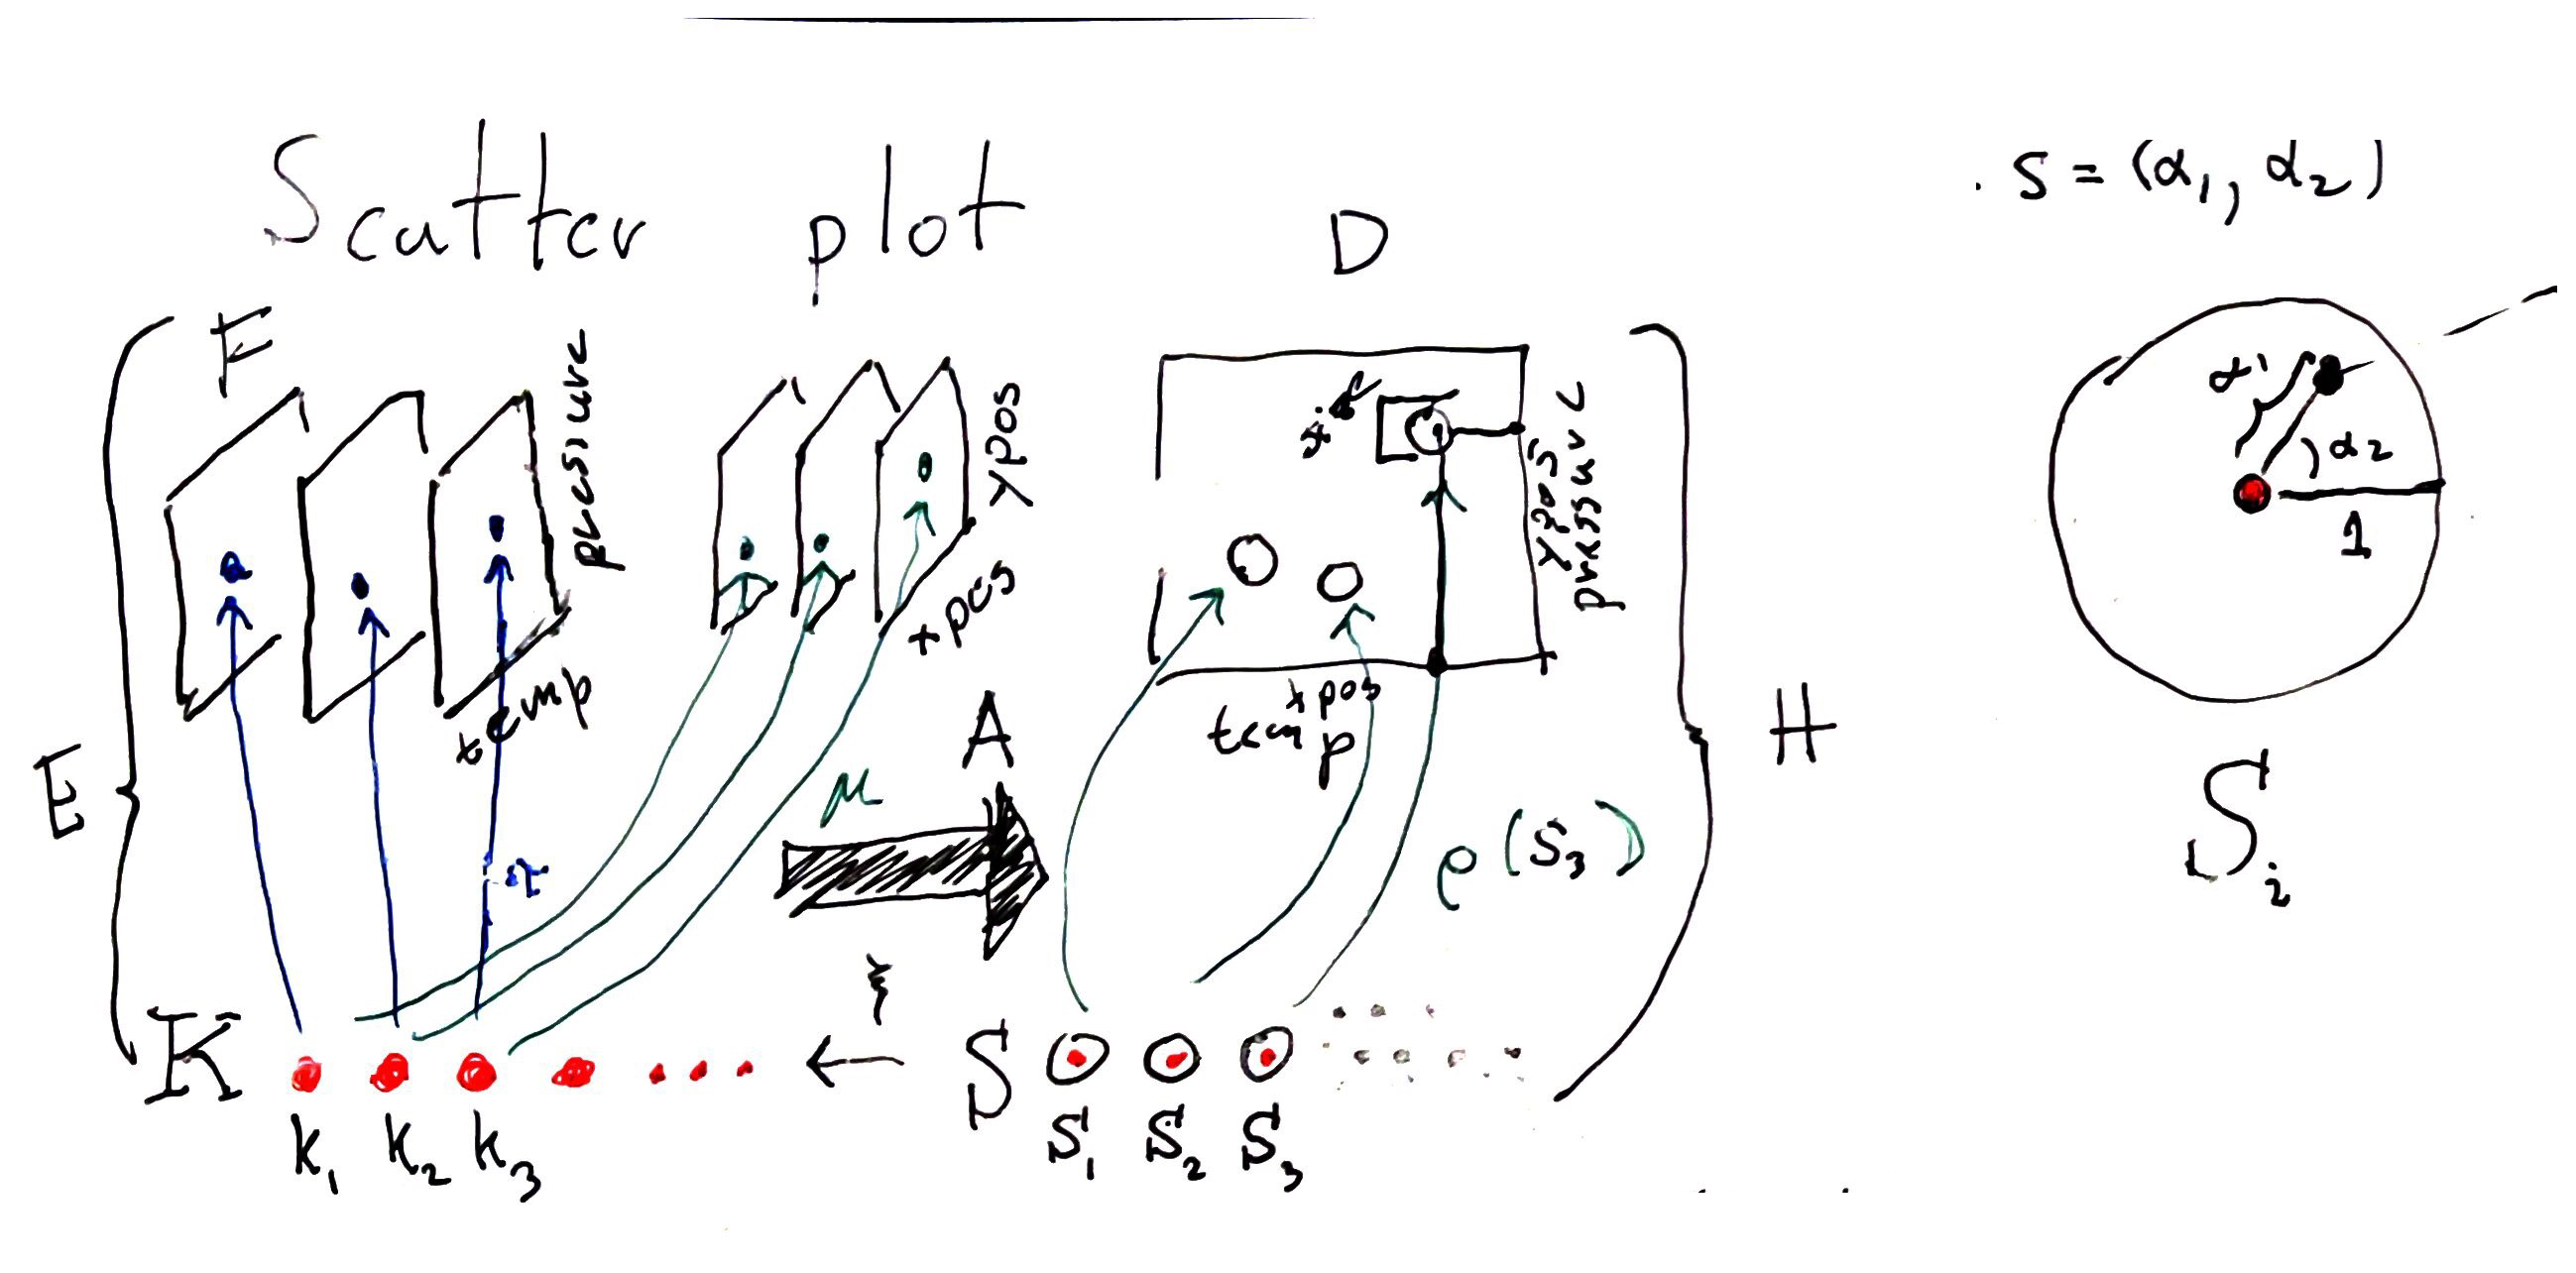
\includegraphics[width=\textwidth]{figures/math/scatter.png}
    \label{fig:artist_scatter}
\end{figure}

\begin{equation}
Q(xpos, ypos)(\alpha_{1}, \alpha_{2}) 
\end{equation}

Given a defaut color of black, $\rho_{RGB} = (0,0,0)$. The position of this swatch of color can be computed relative to the location on the disc $S_{i}$ as shown in figure~\ref{fig:artist_scatter}:
\begin{align}
x &= size\bullet \alpha_1 \bullet \cos(\alpha_2) + xpos\\
y &= size\bullet \alpha_1 \bullet \sin(\alpha_2) + ypos
\end{align}

such that $\rho(s) = (x, y, 0, 0, 0)$ where $s$ is the region in $H$. 

\paragraph{Q: line plot}\mbox{} \\
\label{sec:artist_example_line}
\begin{figure}[H]
    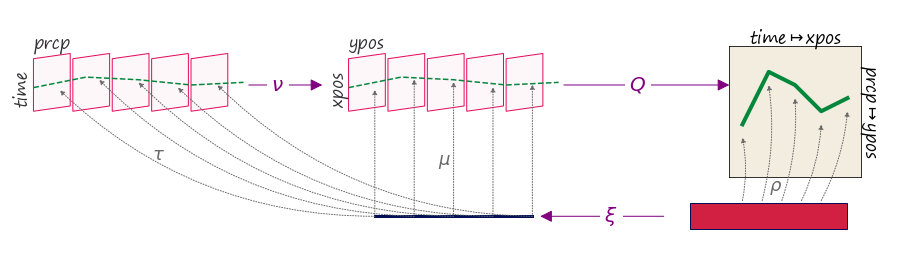
\includegraphics[width=\textwidth]{figures/math/line.png}
    \label{fig:artist_line}
\end{figure}

The line plot shown in fig~\ref{fig:artist_scatter} exemplifies the need for the jet discussed in section~\ref{sec:sheaf_stalk}
(needs the normal to push up/down against the normal)

\begin{equation}
    Q(xpos, \hat{n_{1}}, ypos, \hat{n_{2}})(\alpha_1, \alpha_2)
\end{equation}

where the magnitude of the thickness is 
\begin{equation}
    \lvert n \rvert = \sqrt{{n_{1}}^2 + {n_{2}}^2}
\end{equation}
such that the components are 
\begin{equation}
    \hat{n_{1}} = \frac{n_1}{\lvert n \rvert}, \; \hat{n_{2}} = \frac{n_2}{\lvert n \rvert}
\end{equation}
    
%% only alpha1 exists on the data side
which yields components of $\rho(s)$:
\begin{align}
 x = xpos(\xi(\alpha_1)) &+ \alpha_2\hat(n_1)(\xi(\alpha_1)) \\
 y = ypos(\xi(\alpha_1)) &+ \alpha_2\hat(n_2)(\xi(\alpha_2)) 
\end{align}


\paragraph{Q: heatmap}\mbox{} \\
\label{sec:artist_example_heatmap}
\begin{figure}[H]
    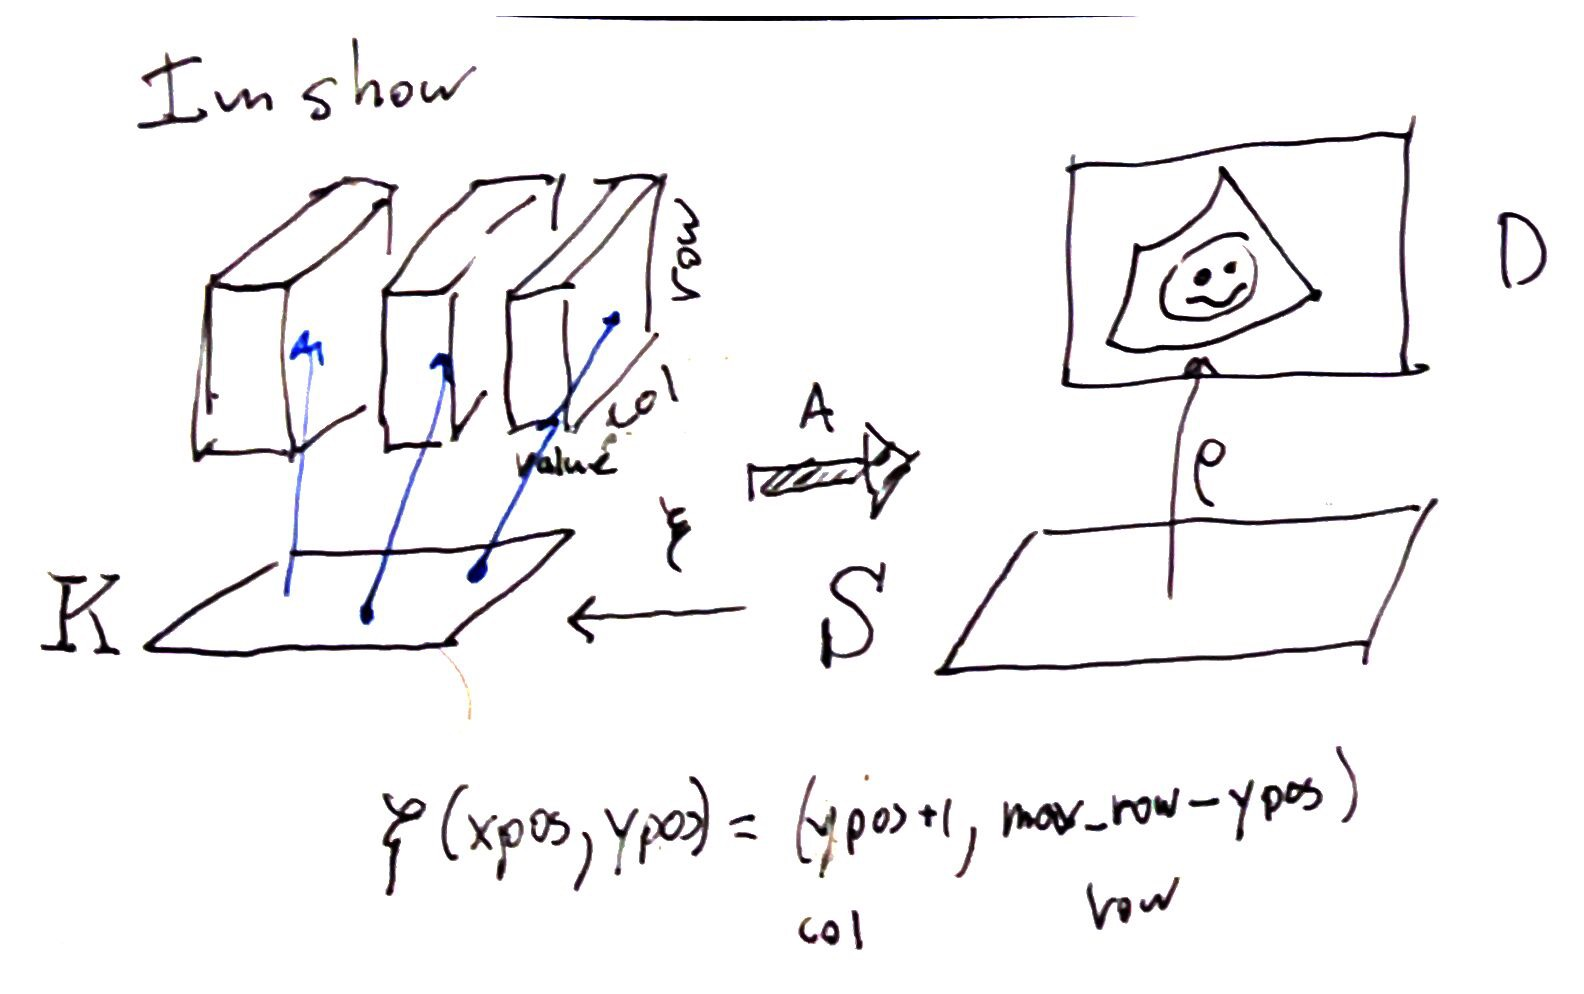
\includegraphics[width=\textwidth]{figures/math/heatmap.png}
    \label{fig:artist_heatmap}
\end{figure}
The heatmap in figure~\ref{fig:artist_heatmap} 
\begin{equation}
Q(xpos, ypos, color)
\end{equation}
has in the simple case a direct lookup into $K$ to obtain the $\mu = (x,y,c)$ values that are mapped into 
(arrays are upside down, x is y, is x) - $\xi$ is about translating indices from data to visual alignment
\begin{align}
D_{RGB} &= color(\xi(\alpha_1, \alpha_2))
D_x & = xpos(\xi(\alpha_1, \alpha_2))
D_y &= ypos(\xi(\alpha_1, \alpha_2))
\end{align}
through $\rho$. 


\subsection{Making the fiber bundle computable}
\label{sec:triangulization}
\note{HAVE NOT REACHED HERE TO EDIT YET}

\begin{figure}[H]
    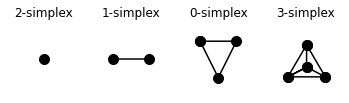
\includegraphics{figures/math/simplex.png}
    \caption{Simplices can encode the connectivity of the data, from fully disconnected (0 simplex) records to all records are connected to at least 3 others}
    \label{fig:triangle_simplex}
\end{figure}

One way to build flexible $\xi$ is to choose a consistent way of representing $K$. In our draft implementation of the data as fiber bundle model, we triangularize $K$ using complexes of the simplicies shown in figure~\ref{fig:triangle_simplex} such that $\xi$ consistently yields some combination of vertexes, edges, and faces. This gives a common data indexing structure on which to build components that could potentially be reused across $Q$.

By using simplicies, we can then encode the following indexing structure on $\tau$
\begin{align*}
    \textbf{vertexes}\;& \tau(k) \text{k= vertex id}\\
    \textbf{edges}\;& \tau(k,\alpha), \text{k = edge id, $\alpha$ = distance along edge} \\
    \textbf{faces}\;& \tau(k,\alpha, \beta), \text{k = face id, $\alpha$ = x on face, $\beta$ = y on face}
\end{align*}

which $\xi$ can use as part of its mapping from visual space back to data space. Path connected components are then sections where $\tau(k_{i},1) = \tau(k_{j},0)$ or the edges of the faces align.  

\subparagraph{Example: Mobius Strip}\mbox{}\\
\begin{figure}[H]
    \label{fig:data_base_transition}
    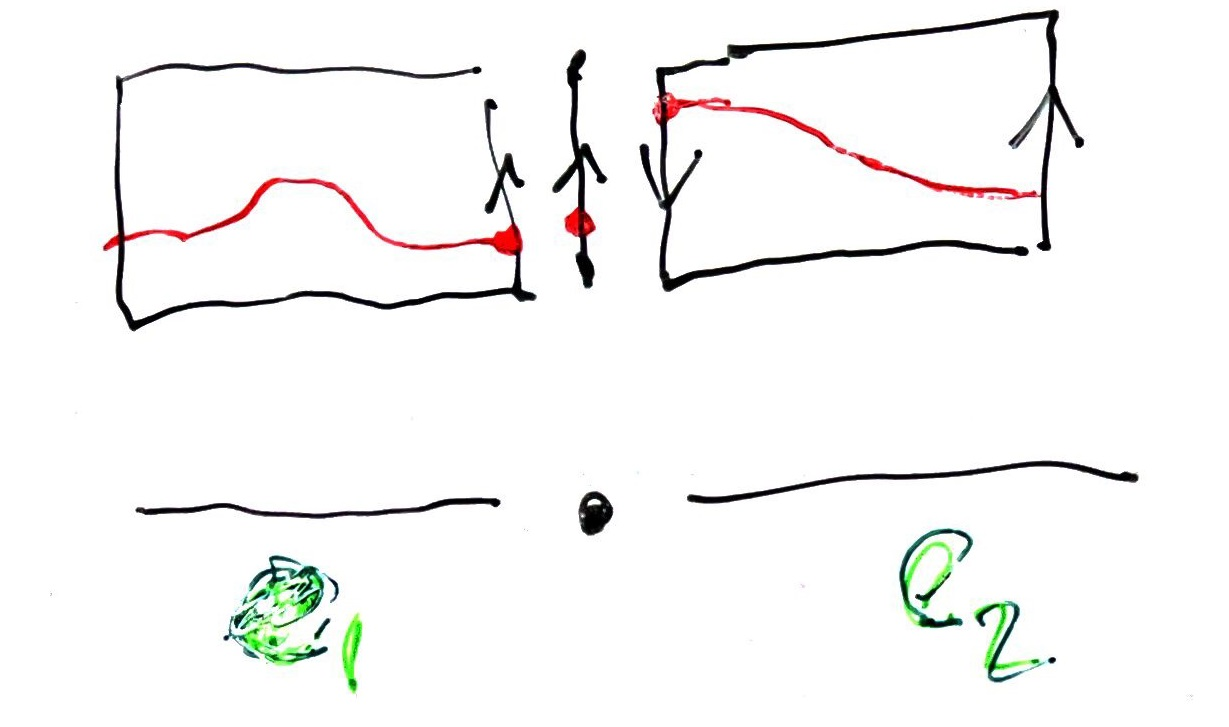
\includegraphics[width=\textwidth]{figures/math/transition_functions.png}
    \caption{Many non-trivial spaces can be made locally trivial by dividing $E$ into locally trivial subspaces and defining transition functions between the edges on K for how to glue the two subspaces such that the sigmas are continuous.}
\end{figure}

 An example of a non-trivial fiber bundle is a mobius strip\cite{find the citation for why};

In figure ~\ref{fig:data_base_transition}, the mobius strip is cut into two rectangular base spaces over $K=\{e_1, e_2\}$. We define transition functions from the fiber to the fiber along the edges of the rectangles such that we can glue these rectangles together to reform the mobius strip. A constraint we impose on the transition functions is that the monoid actions are commutative
%monoid action m*f\mapsto delta(mf)= m*delta(f)

\subparagraph{Example: Torus}\mbox{}\\
\begin{figure}[H]
    \label{fig:triangle_torus}
    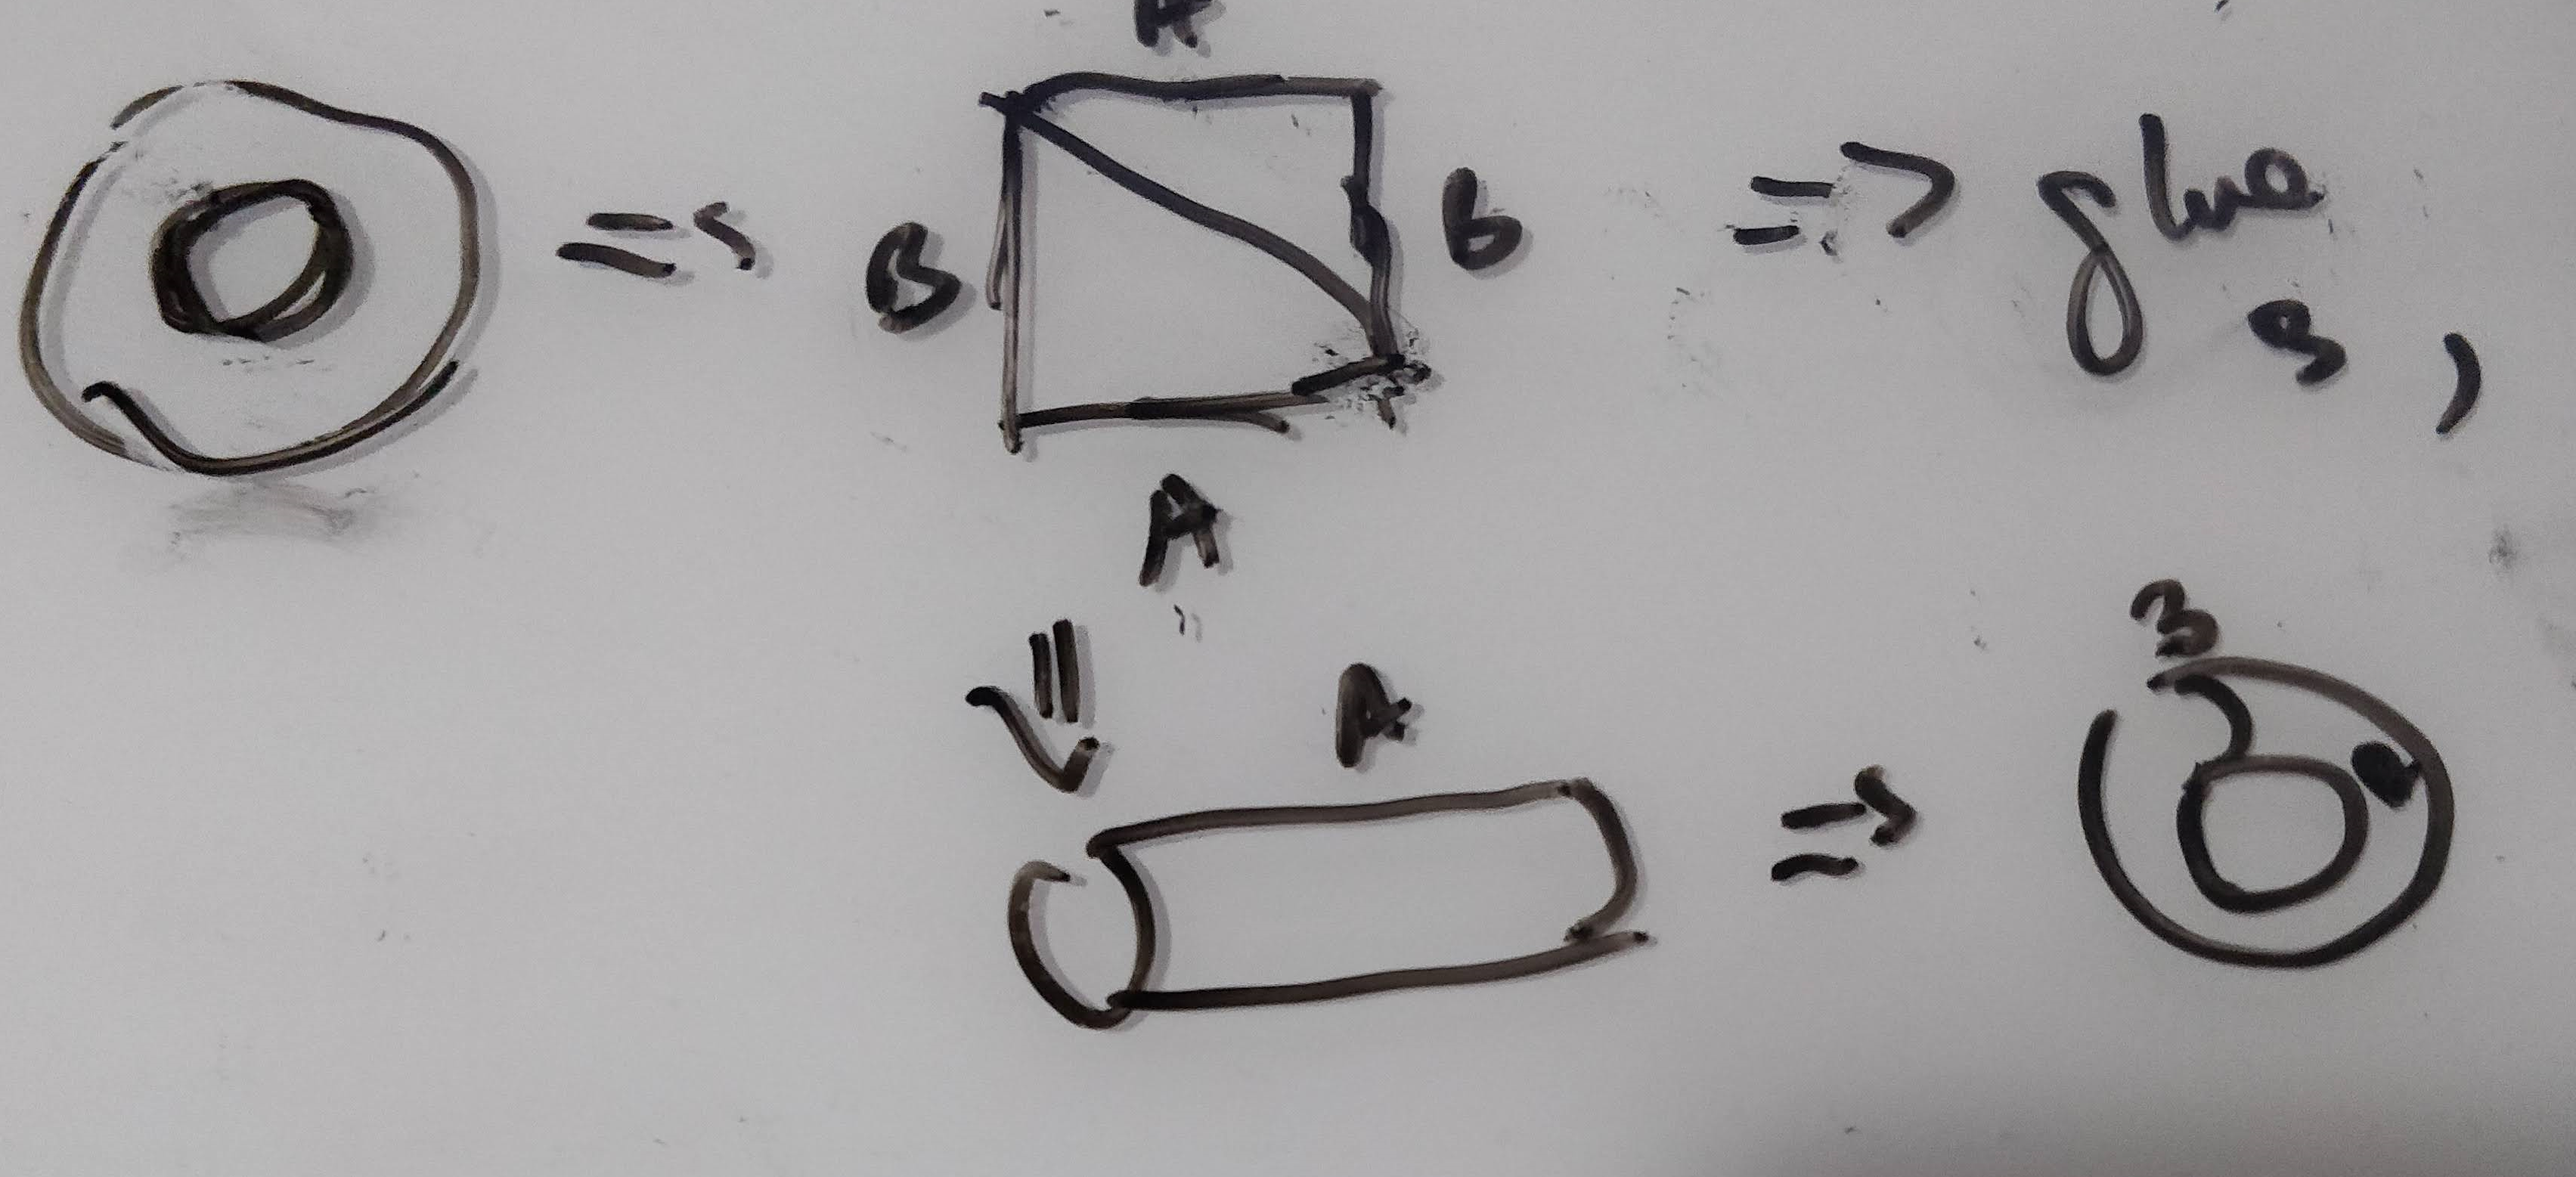
\includegraphics[width=\textwidth]{figures/math/triangle_torus.png}
    \caption{Representation of the base space $K$ of a toridal total space $E$ as two connected 2-simplices.}
\end{figure}

Given data that lies on the toroidal space shown in figure~\ref{fig:triangle_torus}, the torus $E$ base space $K$ can be implemented as a simplacial complex of two 2-simplexes. We unfold the torus into the two triangles that compose the square; the sections on these triangles are $\tau(triangle id k, \alpha, \beta)$. We also put transition functions on the edges such that $A$ can be glued to $A^\prime$ and $B$ to $B^\prime$ to reconstruct the torus. 

\subsubsection{Visual Idioms: Equivalance class of artists}
\note{HAVE NOT REACHED HERE TO EDIT YET}
As formulated above, every artist function $A$ has fixed $\nu$ and generates a distinct graphic $\rho$. It is unfeasible to implement $A$ for every single graphic; instead we implement the equivalence class of artists $\{A \in A^\prime: A_{1} \equiv A_{2}\}$ which is $Q:\Gamma(V) \rightarrow \Gamma(H)$. 

%% Well maybe. I think this is where required components comes in. There is some minimal V where if you didn't have those variables you wouldn't call it a scatter plot .... something like xpos,ypos with K just a descrete set.
%% so V probably can be any V that contains that sub-bundle
%% so if bubble plot is not the same as scatter plot, and something where the colors change based on data is not scatter plot then it is the equivalent class of something with that minimal bundle.
%% But then if you want to include ANYTHING that also maps with X-Y ... then you hit "direct limits" where you limit over all possivle V_big containing V_minimal
%% You still get a map on some A_minimal -> A_big
%% If you know how to visualize with more variables .. you can always fix them.
\end{document}